\documentclass[red, tikz, aspectratio=169, xcolor=dvipsnames]{beamer}
\setbeamertemplate{blocks}[rounded][shadow=false]
\usetheme{Madrid}
\setbeamertemplate{items}[square]
\setbeamertemplate{caption}[numbered]
\usecolortheme{beaver}
\setbeamercolor{frametitle}{bg=white!10!white}

\usefonttheme{professionalfonts}
\setbeamertemplate{itemize item}{\color[rgb]{0.8,0,0}$\blacksquare$}
\setbeamertemplate{itemize subitem}{\color[rgb]{0.8,0,0}$\blacksquare$}
\setbeamertemplate{itemize subsubitem}{\color[rgb]{0.8,0,0}$\blacksquare$}

%Definições de seção
\setcounter{secnumdepth}{3}
\setcounter{tocdepth}{2}

\mode<presentation>{} % https://tex.stackexchange.com/questions/116913/display-the-definition-of-each-items-in-beamer-one-by-one-using-onslide-or-any-m
\usepackage{textcomp}
\usepackage{xkeyval}
\usepackage{todonotes}
\presetkeys{todonotes}{inline}{}

\usepackage{tikzsymbols}
\usepackage{helvet}
\renewcommand{\familydefault}{\sfdefault}
\usepackage{float}
\usepackage[brazil]{babel}
\usepackage[utf8]{inputenc}
\usepackage{graphicx}
\usepackage{url}
\usepackage{subfigure}
\usepackage{mathtools} % setas com texto
\usepackage{multicol}
\usepackage{listings}
\usepackage{scalefnt}
\usepackage{ragged2e}
\usepackage{etoolbox, verbatim}
\usepackage{soul}

\usepackage[linguistics]{forest}
\usepackage[cache=false]{minted}

\usepackage{amsmath}
\usepackage{algorithmic}
\usepackage[linesnumbered,ruled,algo2e]{algorithm2e}

% Listing
\lstset{
	numbers=left,
	stepnumber=1,
	numbersep=5pt,
	numberstyle=\small\color{black},
	basicstyle= \scriptsize,
%	keywordstyle=\color{black},
%	commentstyle=\color{black},
%	stringstyle=\color{black},
	tabsize=2
}

\let\olditem=\item%
\renewcommand{\item}{\olditem \justifying}

\title[Algoritmos e Estrutura de Dados - II]{\textbf{Algoritmos e Estrutura de Dados - II}\\\textit{Estrutura de Dados Espaciais}}
\author[\textit{rodolfolabiapari@decom.ufop.br}]{Rodolfo Labiapari Mansur Guimarães}
\institute[IFMG]{\begin{figure}
			\centering
			
\includegraphics[width=0.1\textwidth]{img/ufop.jpg}
		\end{figure}}
\institute[UFOP]{
	\textit{rodolfolabiapari@decom.ufop.br} -- Lattes: \url{http://goo.gl/MZv4Dc} \\
	Departamento de Computação -- Instituto de Ciências Exatas e Biológicas (ICEB)\\
	Universidade Federal de Ouro Preto (UFOP) \\
	Ouro Preto - MG -- Brasil }

\date{Última Atualização: \today}

\begin{document}


\frame{\titlepage}

\AtBeginSection[]
{
	\begin{frame}
	\frametitle{Sumário}
	\tableofcontents[]
	\end{frame}
}

\AtBeginSubsection[]
{
	\begin{frame}
		\frametitle{Sumário}
		\tableofcontents[
		currentsection,
		currentsubsection,
		hideothersubsections,
		%sectionstyle=show/hiden,
		subsectionstyle=show/shaded, ]
	\end{frame}
}


%\usebackgroundtemplate{
\includegraphics[trim=0cm 0cm 10cm 0cm, width=0.03\textwidth]{img/ufop.jpg}}


\section{Dados Escalares}
	\begin{frame}{Dados Escalares}
		\begin{block}{Definição de Dado Escalar}
			Na matemática, na informática, e na física, uma \textbf{grandeza escalar} é definida quando precisamos de \textbf{um valor numérico} associado a \textbf{uma unidade de medida para caracterizar alguma grandeza}.
		\end{block}
				\pause
				\bigskip
		\begin{itemize}
			\setlength{\itemsep}{0.9em}
			\item \textit{Qual a população de Ouro Preto?}
				Cerca de 74 mil habitantes.
			\item \textit{Quantos alunos a UFOP possui?}
				Corpo Discente, são 9.658 alunos na graduação, sendo 3.363 na modalidade à distância.
				Na pós-graduação, são 434 alunos no mestrado, 121 no doutorado e 500 na especialização.
		\end{itemize}
	\end{frame}

	\begin{frame}{Dados Escalares}
		\begin{table}
			\centering
		    \begin{tabular}{c|c|c|c|c}
		    	\hline 
			    \textbf{Inscrição} & \textbf{Nota} & \textbf{Estado} & \textbf{Cidade}     & \textbf{Curso}                \\\hline \hline 
			    00467354  & 47,8 & MG     & VICOSA     & ADMINISTRACAO        \\\hline 
			    00085820  & 52,0 & MG     & UBERLANDIA & DIREITO              \\\hline 
			    00015022  & 51,0 & MG     & ALFENAS    & ENGENHARIA CIVIL     \\\hline 
			    00403068  & 08,0 & MG     & VARGINHA   & ENGENHARIA QUIMICA   \\\hline 
			    00130230  & 36,3 & MG     & UBERABA    & MEDICINA VETERINARIA \\\hline 
		    \end{tabular}
		\end{table}
	
		\begin{itemize}
			\item Com esses dados, é possível responder:
			\begin{itemize}
				\it
				\setlength{\itemsep}{1.2em}
				\item Qual a média das notas dos alunos que moram na proximidade de Uberlândia?
				\item Quais os alunos que moram numa distância maior à 300km da capital do estado?
			\end{itemize}
		\end{itemize}
	\end{frame}


\section{Dados Espaciais (Geográficos)}
	\begin{frame}{Dados Espaciais}
		\begin{table}
			\centering
			\footnotesize
		    \begin{tabular}{c|c|c|c|c|c|c}
			    \hline 
			    \textbf{Inscrição} & \textbf{Nota} & \textbf{Estado} & \textbf{Cidade}     & \textbf{Curso}                & \textbf{Latitude} & \textbf{Longitude} \\ \hline \hline 
			    00467354  & 47,8 & MG     & VICOSA     & ADMINISTRACAO        & -20.7548659        & -42.8785788         \\\hline 
			    00085820  & 52,0 & MG     & UBERLANDIA & DIREITO              & -18.9146078        & -48.2753801         \\\hline 
			    00015022  & 51,0 & MG     & ALFENAS    & ENGENHARIA CIVIL     & -21.4261129        & -45.9481612         \\\hline 
			    00403068  & 08,0 & MG     & VARGINHA   & ENGENHARIA QUIMICA   & -21.5560521        & -45.4368421         \\\hline 
			    00130230  & 36,3 & MG     & UBERABA    & MEDICINA VETERINARIA & -19.7473748        & -47.9391625         \\\hline 
		    \end{tabular}
		\end{table}
	
			\bigskip
		\begin{itemize}
			\item Com esses dados, é possível responder anteriores:
			\begin{itemize}
				\setlength{\itemsep}{1.2em}
				\it
				\item Qual a média das notas dos alunos que moram na proximidade de Uberlândia?
				\item Quais os alunos que moram numa distância maior à 300km da capital do estado?
			\end{itemize}
		\end{itemize}
	\end{frame}

	\begin{frame}{Relações entre dados e espaço}
		\begin{itemize}
			\setlength{\itemsep}{1.2em}
			\item Localização:
			\begin{itemize}
				\item Existe uma cidade chamada ``São Paulo''?
				\item Existe uma cidade em -23.5505199, -46.6333094?
			\end{itemize}
			
			\item Vizinhança:
			\begin{itemize}
				\item Qual a cidade mais próxima à São Paulo?
			\end{itemize}
			
			\item Extensão:
			\begin{itemize}
				\item Qual o perímetro de São Paulo?
				\item Qual a área de São Paulo?
			\end{itemize}
		\end{itemize}
	\end{frame}
	
	\begin{frame}
		\begin{figure}
			\centering
			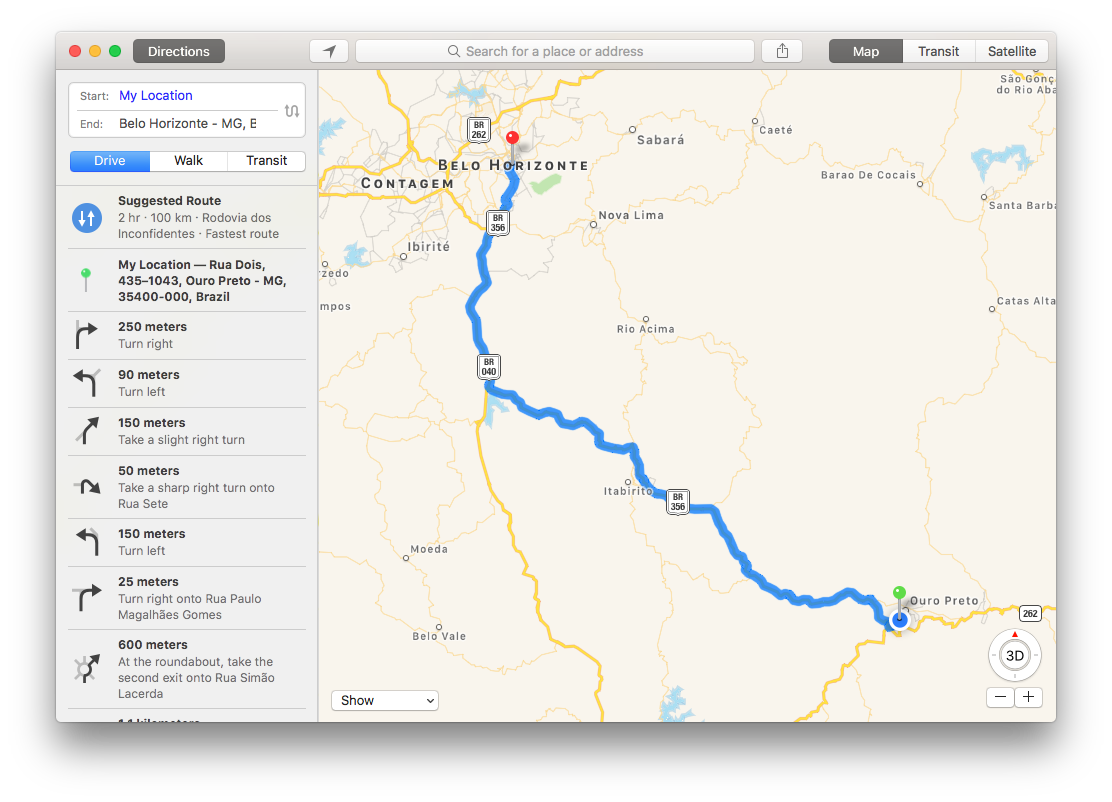
\includegraphics[width=0.80\textwidth]{img/localizacao_1.png}
		\end{figure}
	\end{frame}
	
	\begin{frame}
		\begin{figure}
			\centering
			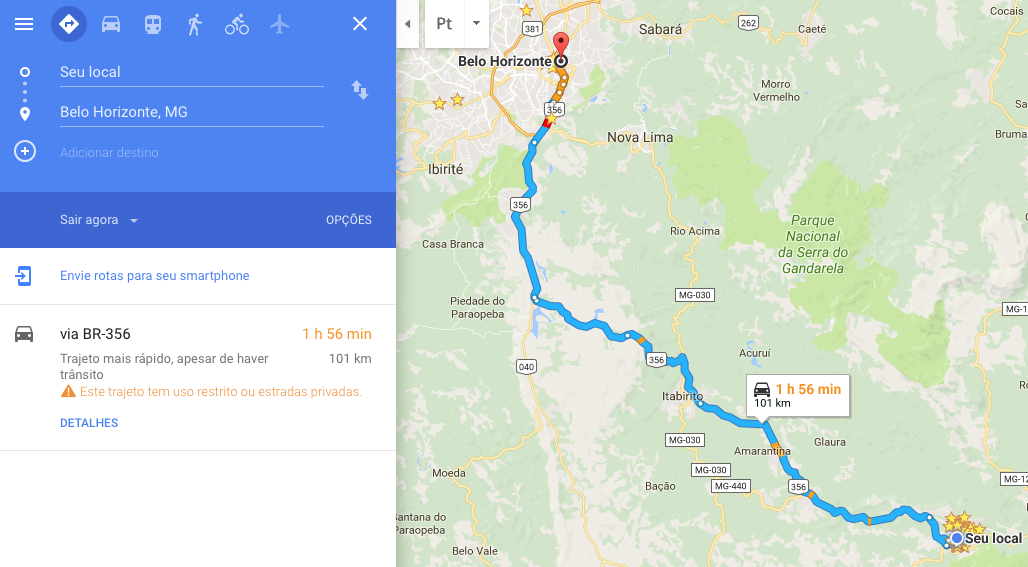
\includegraphics[width=0.90\textwidth]{img/localizacao_2.png}
			%\caption{Dados vetoriais.}
		\end{figure}
	\end{frame}
	
	\begin{frame}
		\begin{figure}
			\centering
			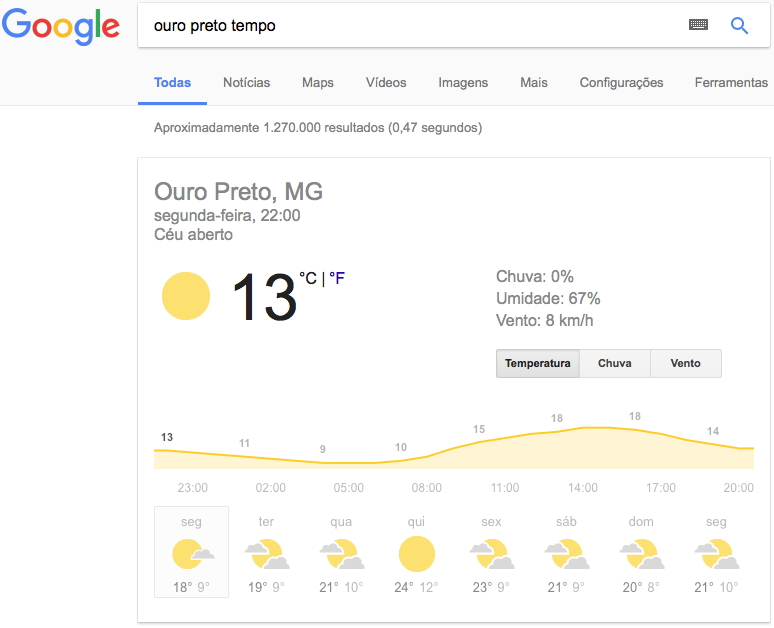
\includegraphics[width=0.7\textwidth]{img/localizacao_4.png}
		\end{figure}
	\end{frame}
	
	\begin{frame}
		\begin{figure}
			\centering
			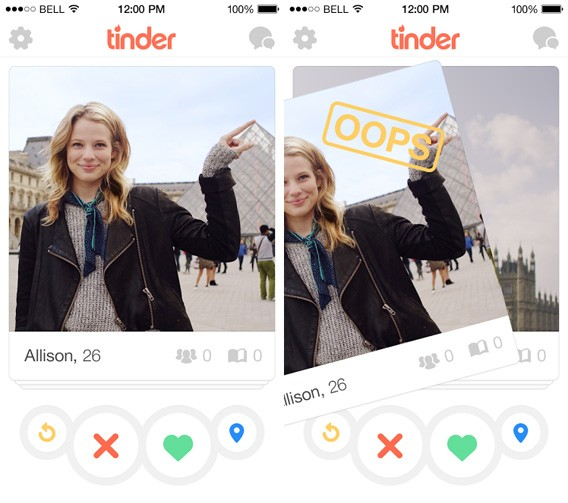
\includegraphics[width=0.65\textwidth]{img/localizacao_3.jpg}
		\end{figure}
	\end{frame}
	
	\begin{frame}
		\begin{figure}
			\centering
			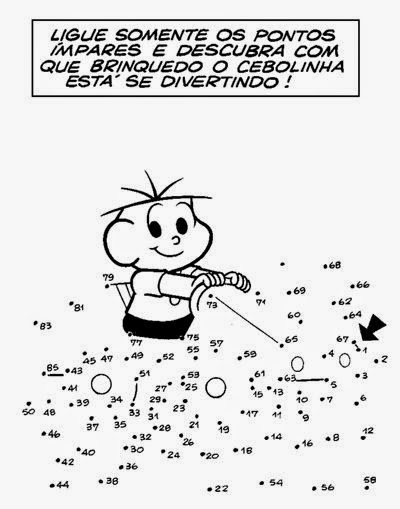
\includegraphics[width=0.42\textwidth]{img/uso_1.jpg}
		\end{figure}
	\end{frame}
	
	\begin{frame}
		\begin{figure}
			\centering
			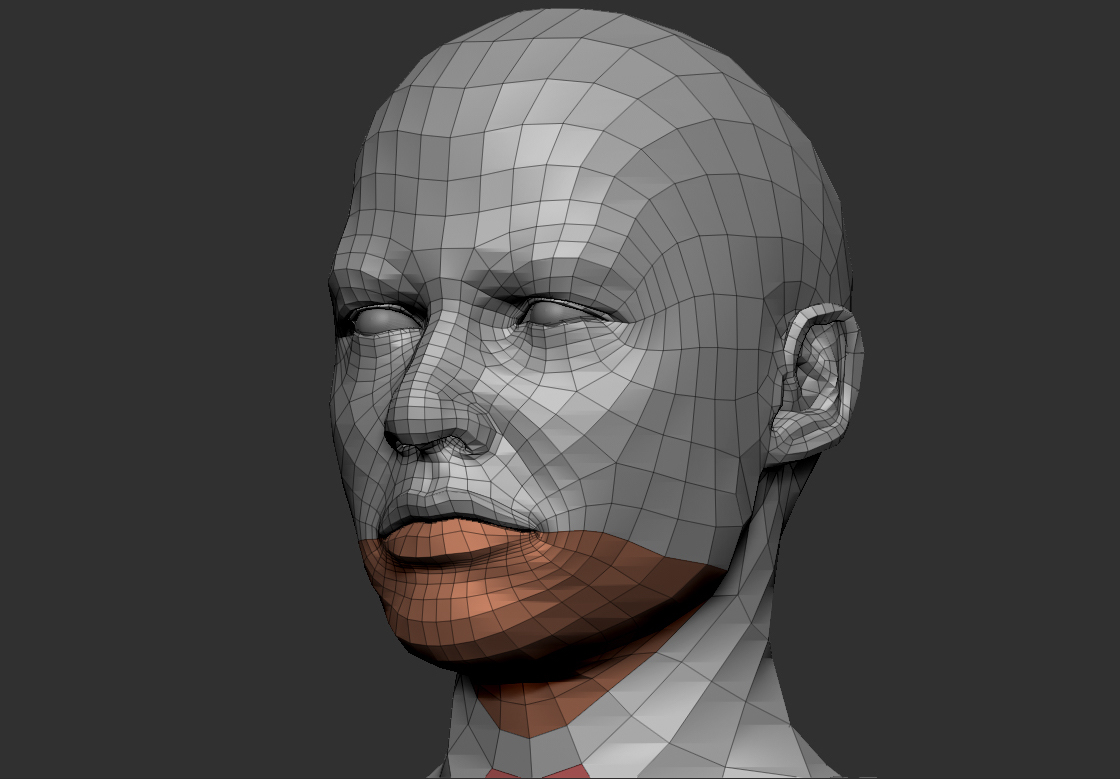
\includegraphics[width=0.72\textwidth]{img/uso_2.jpg}
		\end{figure}
	\end{frame}


\section{Banco de Dados}
	\subsection{Conceituação}
		\begin{frame}{Introdução à Banco de Dados}
			\begin{block}{Conceito}
				Banco de dados é uma coleção de dados relacionados, projetados para uma finalidade específica.
			\end{block}
				\pause
				\bigskip
			Exemplo de Banco de Dados:
			\begin{table}
				\centering
				\begin{tabular}{c|c|c|c|c}
					\hline 
					\textbf{Inscrição} & \textbf{Nota} & \textbf{Estado} & \textbf{Cidade}     & \textbf{Curso}                \\\hline \hline 
					00467354  & 47,8 & MG     & VICOSA     & ADMINISTRACAO        \\\hline 
					00085820  & 52,0 & MG     & UBERLANDIA & DIREITO              \\\hline 
					00015022  & 51,0 & MG     & ALFENAS    & ENGENHARIA CIVIL     \\\hline 
					00403068  & 08,0 & MG     & VARGINHA   & ENGENHARIA QUIMICA   \\\hline 
					00130230  & 36,3 & MG     & UBERABA    & MEDICINA VETERINARIA \\\hline 
				\end{tabular}
			\end{table}
		\end{frame}

		\begin{frame}{Aplicações de um Banco de Dados Comum}
			\begin{itemize}
				\setlength{\itemsep}{1em}
				\item \textbf{Bancos:} depósito ou retirada de fundos da conta bancária;
				\item \textbf{Hotéis:} reservas de quartervas de quartos;
				\item \textbf{Empresas aéreas:} compra e reserva de passagens;
				\item \textbf{Bibliotecas:} consulta ao acervo;
				\item \textbf{Supermercados:} identificação dos produtos comprados, controle do estoque;
				\item \textbf{Lojas virtuais:} clientes e produtos vendidos pelo site;
				\item \textbf{Redes sociais:} fotografias, postagens, curtidas, localização.
			\end{itemize}
		\end{frame}

	\subsection{Banco de Dados Espaciais}

		\begin{frame}{SGBD e BDG}
			%http://www.infoescola.com/informatica/banco-de-dados-geograficos/
			\begin{itemize}
				\setlength{\itemsep}{1em}
				\item Para gerência desses dados, utiliza-se softwares chamados \textbf{Sistemas Gerenciadores de Banco de Dados (SGBDs)}. 
				\begin{itemize}
					\item São exemplos de programas desse tipo: PostgreSQL, MySQL, Access e Oracle.
				\end{itemize}
				
				\item Requisito fundamental hoje nos SGBDs:
				\begin{itemize}
					\item Manipulação dos dados espaciais.
				\end{itemize}
				
				\item \textbf{Banco de Dados Geográficos (BDG)}\footnote{Também são chamados de \textbf{Banco de Dados Espaciais (BDE)}.}, possui o diferencial de suportar dados geométricas em suas tabelas.
	
				\item Possibilita a realização de cálculos como áreas, distâncias e centróides, além de realizar a geração de buffers (zona de influência) e outras operações entre as geometrias.
			\end{itemize}
		\end{frame}

		\begin{frame}{SGBD e BDG}
			%http://www.infoescola.com/informatica/banco-de-dados-geograficos/
			\begin{itemize}
				\item Ao construir um Banco de Dados Geográficos será possível realizar consultas tais como:
	
				\begin{itemize}
					\setlength{\itemsep}{1.2em}
					\item \textit{Que cidades são vizinhas ao município de Ouro Preto?}
					\item \textit{Que municípios são cortados pela BR-040?”}
					\item \textit{Que distância entre a comunidade rural $x$ e a escola mais próxima?”}
				\end{itemize}
			\end{itemize}
		\end{frame}

		\begin{frame}{Aplicações de um Banco de Dados Geográfico}
			%http://www.infoescola.com/informatica/banco-de-dados-geograficos/
			\begin{itemize}
				\setlength{\itemsep}{0.9em}
	
				\item Por exemplo os \textit{softwares}:
				\begin{enumerate}
					\setlength{\itemsep}{0.3em}
					\item Sistema de Informação Geográfica (Cartografia);
					\item CAD (Computer-Aided Design);
					\item Robótica;
					\item Bancos tradicionais na qual um registro com $k$ atributos corresponde a um ponto no espaço $k-d$ onde $d$ é a dimensão;
					\item Banco temporal, onde o tempo pode ser considerado uma dimensão a mais;
				\end{enumerate}

				\item Fazendo processamentos como:
				\begin{enumerate}
					\setlength{\itemsep}{0.3em}
					\item Medir distâncias, perímetro, áreas;
					\item Calcular a conectividade e o caminho mais curto entre dois pontos;
					\item Analisar pontos e linhas dentro de um polígono; 
					\item Realizar buscar por região (intervalo);
					\item etc.
				\end{enumerate}
			\end{itemize}
		\end{frame}

		\begin{frame}{Outras Aplicações}
			Fora da área de geoprocessamento, QuadTree pode ser usado em:
			\begin{itemize}
				\setlength{\itemsep}{1.5em}
				\item Fotografias e imagens;
				\begin{enumerate}
					\item Algoritmos de compressão de imagens;
					\item Correção de deformações em fotos como olhos avermelhados;
					\item Rotação de imagens.
				\end{enumerate}
				
				\item Medicina:
				\begin{enumerate}
					\item Ecografias, identificando tumores pela cor na imagem.
				\end{enumerate}
				
				\item Video-chamadas:
				\begin{enumerate}
					\item Trasmitindo somente o que foi alterado na imagem.
				\end{enumerate}
				
				\item Jogos:
				\begin{enumerate}
					\item Detecção de colisão.
				\end{enumerate}
			\end{itemize}
		\end{frame}

\section{Estruturas de Dados Espaciais}	

	\subsection{Representação de Dados Espacias}
	
		\begin{frame}{Representação de Dados Vetoriais}
			\begin{figure}
				\centering
				\label{fig:vetorial_data}
				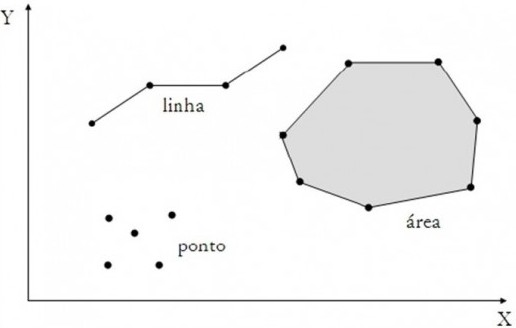
\includegraphics[width=0.56\textwidth]{img/vetorial_data.jpg}
				%\caption{Dados vetoriais.}
			\end{figure}
		
			\begin{itemize}
				\item Pelo menos 1 par de coordenadas
				\item Representados por pontos, linhas (arcos e demais elementos lineares) ou polígonos (áreas), etc.
			\end{itemize}
		\end{frame}

		\begin{frame}
			\begin{figure}
				\centering
				\label{fig:vetorial_data_2}
				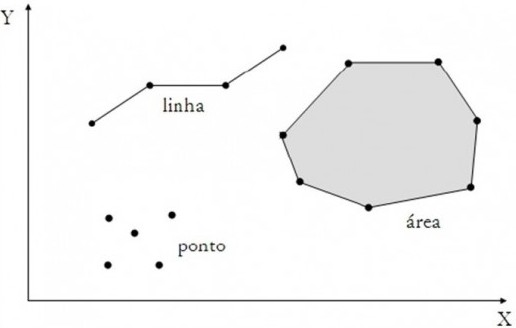
\includegraphics[width=0.56\textwidth]{img/vetorial_data.jpg}
				%\caption{Dados vetoriais.}
			\end{figure}
		
			\begin{itemize}
				\item Possíveis representações:
				\begin{itemize}
					\setlength{\itemsep}{0.7em}
					\item \textbf{Pontos:} localização de crimes ou ocorrências de doenças;
					\item \textbf{Linhas} representação traçado de rios e semelhantes;
					\item \textbf{Polígonos} lotes de uma quadra até continentes. 
				\end{itemize}
			\end{itemize}
		\end{frame}
	
		\begin{frame}{Representação de Dados Matricial}
			\vspace{-10px}
			\begin{figure}
				\centering
				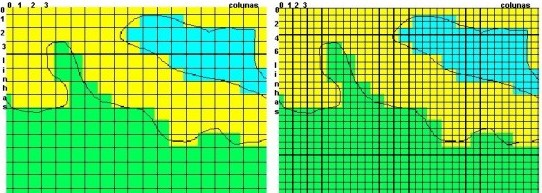
\includegraphics[width=0.85\textwidth]{img/matricial_data.jpg}
				\caption{\textit{Raster} (Contorno).}
			\end{figure}
		
			\begin{itemize}
			\setlength{\itemsep}{0.4em}
			\item Cruzamento dos atributos das linhas e colunas:
			\begin{itemize}
				\item Cada célula possui uma informação.
			\end{itemize}
		
			\item Observe que a Figura da direita tem melhor resolução espacial.
			\end{itemize}
		\end{frame}
	
	
		\begin{frame}
			\vspace{-10px}
			\begin{figure}
				\centering
				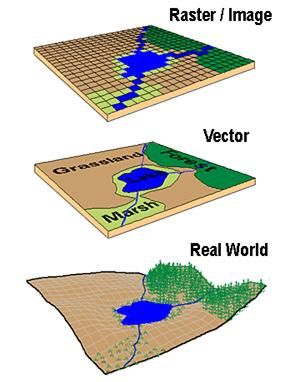
\includegraphics[width=0.47\textwidth]{img/spatial.jpg}
				\caption{\textit{Raster} (Contorno).}
			\end{figure}
		\end{frame}


	\subsection{Estruturas Já Conhecidas}
	
		\begin{frame}{Tabela Hash}
			\begin{figure}
				\centering
				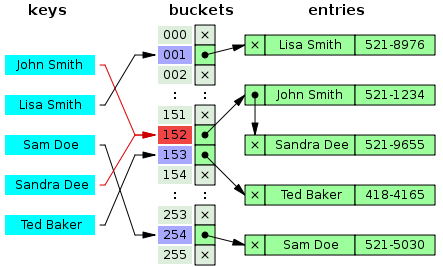
\includegraphics[width=0.7\textwidth]{img/hash.png}
				%\caption{Dados vetoriais.}
			\end{figure}
			\begin{itemize}
				\item Não atende às consultas de intervalos.
			\end{itemize}
		\end{frame}
		
		\begin{frame}{Árvores Binárias e \textit{n}-árias}
			\begin{figure}
				\centering
				\label{fig:uso_4}
				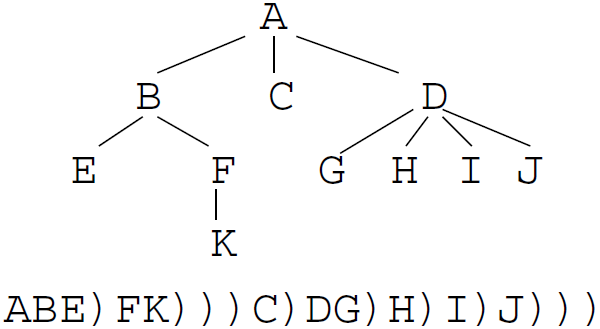
\includegraphics[width=0.72\textwidth]{img/n-tree.png}
				%\caption{Dados vetoriais.}
			\end{figure}
			\begin{itemize}
				\item Trata apenas uma dimensão, ou seja uma outra representação de vetor.
			\end{itemize}
		\end{frame}
	
		\begin{frame}
			\begin{figure}
				\centering
				\label{fig:vetorial_data_23}
				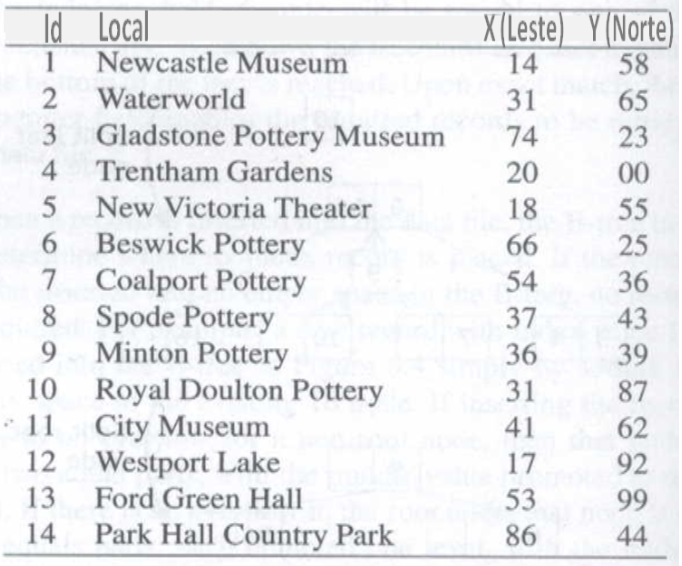
\includegraphics[width=0.58\textwidth]{img/address.png}
				%\caption{Dados vetoriais.}
			\end{figure}
					\pause
			\begin{itemize}
				\item Quais os dados do no intervalo \texttt{(20, 20)} e \texttt{(40, 50)}?
			\end{itemize}
		\end{frame}
	
		\begin{frame}[fragile]{Consulta Linear de Intervalo}
			\begin{columns}
				\begin{column}{0.44\textwidth}
					\begin{figure}
						\centering
						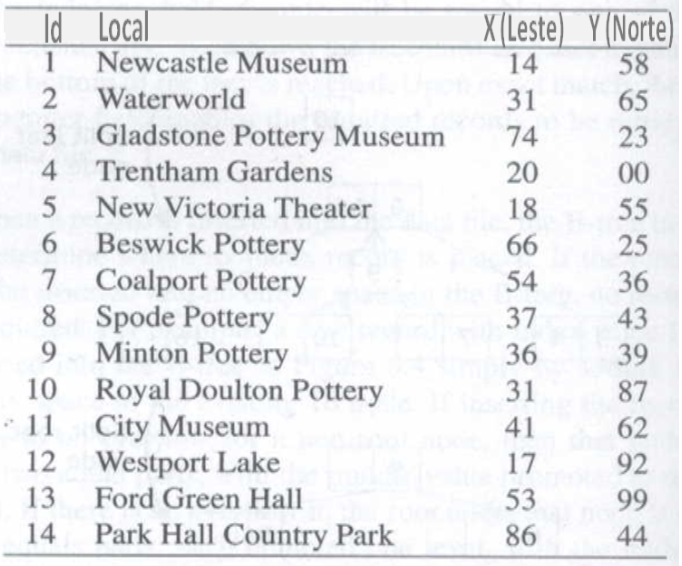
\includegraphics[width=1\textwidth]{img/address.png}
						%\caption{Dados vetoriais.}
					\end{figure}
				\end{column}
				\begin{column}{0.48\textwidth}
					\begin{algorithm2e}[H]
						\While{Existe registros à Examinar}{
							Lê o próximo Registro\;
							\If{Verifica se x está na faixa}{
								\If{Verifica se y está na faixa}{
									Recupera o Registro}}}
						\caption{Interval Search - $\mathcal{O}(n)$} 
					\end{algorithm2e}
				\end{column}
			\end{columns}
		\end{frame}

	
	\subsection{QuadTree}	
	
		\begin{frame}{Propriedades Gerais da QuadTree}
			\begin{itemize}
				\setlength{\itemsep}{1.3em}
				\item Técnica bastante simples;
				\item Extensão multidimensional da árvore de busca binária;
				\item O índice é representado como uma árvore quaternária
				\begin{itemize}
					\setlength{\itemsep}{0.8em}
					\item O espaço de busca é decomposto em quadrantes
					\begin{itemize}
						\item Nas quais são nomeados por: Noroeste, Nordeste, Sudeste e Sudoeste.
					\end{itemize}
				
					\item Pontos são armazenados em nós internos;
					\item Para $n$ pontos, espera-se uma altura de $\mathcal{O}(\log n)$;
					\item Acelera o acesso a dados num plano 2 dimensões;
				\end{itemize}
			\end{itemize}
		\end{frame}



		\subsubsection{Point QuadTree}
		
			\begin{frame}[fragile]{Point QuadTree}{Estruturas de Dados Básicas}
				\begin{columns}
					\begin{column}{0.48\textwidth}
						\centering
						\begin{minted}{c}
struct PQNo {
	PQNo *filhos[4];
	int x;
	int y;
};
						\end{minted}
					\end{column}
					\begin{column}{0.5\textwidth}
						\centering
						\fbox{
							\begin{forest}
								[\texttt{(x,y)}
								[NO]
								[NE]
								[SO]
								[SE]
								]
						\end{forest}}
					\end{column}
				\end{columns}
			\end{frame}

 


			\begin{frame}[fragile]{Point QuadTree}{Exemplo Prático}
				\centering
				\vspace{-40px}
				\begin{columns}
					\begin{column}{0.48\textwidth}
						\centering
						\begin{tabular}{|c|c|}
							\hline 
							NO (-,+) & NE (+,+) \\ 
							\hline 
							SO (-,-) & SE (+,-) \\ 
							\hline 
						\end{tabular} 
					\end{column}
					\begin{column}{0.5\textwidth}
						\centering
						\fbox{
							\begin{forest}
								[\texttt{(x,y)}
								[NO]
								[NE]
								[SO]
								[SE]
								]
						\end{forest}}
					\end{column}
				\end{columns}
				\vspace{10px}
				
				\fcolorbox{red}{white}{\texttt{\st{(35,40)}, (50,10), (60,75), (80,65), (85,15), (05,45), (25,35), (90,05)}}
				\vspace{10px}
				
				\begin{minipage}{\textwidth}
					\centering
					
					\begin{forest}
						[\texttt{(35,40)}
						[.
						[x]
						[x]
						[x]
						[x]
						]
						[.
						[x]
						[x]
						[x]
						[x]
						]
						[.
						[x]
						[x]
						[x]
						[x]
						]
						[.
						[x]
						[x]
						[x]
						[x]
						]
						]
					\end{forest}
				\end{minipage}
			\end{frame}
			
			\begin{frame}[fragile]{Point QuadTree}{Exemplo Prático}
				\centering
				\vspace{-40px}
				\begin{columns}
					\begin{column}{0.48\textwidth}
						\centering
						\begin{tabular}{|c|c|}
							\hline 
							NO (-,+) & NE (+,+) \\ 
							\hline 
							SO (-,-) & SE (+,-) \\ 
							\hline 
						\end{tabular} 
					\end{column}
					\begin{column}{0.5\textwidth}
						\centering
						\fbox{
							\begin{forest}
								[\texttt{(x,y)}
								[NO]
								[NE]
								[SO]
								[SE]
								]
						\end{forest}}
					\end{column}
				\end{columns}
				\vspace{10px}
				
				\fcolorbox{red}{white}{\texttt{\st{(35,40)}, \st{(50,10)}, (60,75), (80,65), (85,15), (05,45), (25,35), (90,05)}}
				\vspace{10px}
				
				\begin{minipage}{\textwidth}
					\centering
					
					\begin{forest}
						[\texttt{(35,40)}
						[.
						[x]
						[x]
						[x]
						[x]
						]
						[.
						[x]
						[x]
						[x]
						[x]
						]
						[.
						[x]
						[x]
						[x]
						[x]
						]
						[\texttt{(50,10)}
						[x]
						[x]
						[x]
						[x]
						]
						]
					\end{forest}
				\end{minipage}
			\end{frame}
			
			\begin{frame}[fragile]{Point QuadTree}{Exemplo Prático}
				\centering
				\vspace{-40px}
				\begin{columns}
					\begin{column}{0.48\textwidth}
						\centering
						\begin{tabular}{|c|c|}
							\hline 
							NO (-,+) & NE (+,+) \\ 
							\hline 
							SO (-,-) & SE (+,-) \\ 
							\hline 
						\end{tabular} 
					\end{column}
					\begin{column}{0.5\textwidth}
						\centering
						\fbox{
							\begin{forest}
								[\texttt{(x,y)}
								[NO]
								[NE]
								[SO]
								[SE]
								]
						\end{forest}}
					\end{column}
				\end{columns}
				\vspace{10px}
				
				\fcolorbox{red}{white}{\texttt{\st{(35,40)}, \st{(50,10)}, \st{(60,75)}, (80,65), (85,15), (05,45), (25,35), (90,05)}}
				\vspace{10px}
				
				\begin{minipage}{\textwidth}
					\centering
					
					\begin{forest}
						[\texttt{(35,40)}
						[.
						[x]
						[x]
						[x]
						[x]
						]
						[\texttt{(60,75)}
						[x]
						[x]
						[x]
						[x]
						]
						[.
						[x]
						[x]
						[x]
						[x]
						]
						[\texttt{(50,10)}
						[x]
						[x]
						[x]
						[x]
						]
						]
					\end{forest}
				\end{minipage}
			\end{frame}
			
			\begin{frame}[fragile]{Point QuadTree}{Exemplo Prático}
				\centering
				\vspace{-40px}
				\begin{columns}
					\begin{column}{0.48\textwidth}
						\centering
						\begin{tabular}{|c|c|}
							\hline 
							NO (-,+) & NE (+,+) \\ 
							\hline 
							SO (-,-) & SE (+,-) \\ 
							\hline 
						\end{tabular} 
					\end{column}
					\begin{column}{0.5\textwidth}
						\centering
						\fbox{
							\begin{forest}
								[\texttt{(x,y)}
								[NO]
								[NE]
								[SO]
								[SE]
								]
						\end{forest}}
					\end{column}
				\end{columns}
				\vspace{10px}
				
				\fcolorbox{red}{white}{\texttt{\st{(35,40)}, \st{(50,10)}, \st{(60,75)}, \st{(80,65)}, (85,15), (05,45), (25,35), (90,05)}}
				\vspace{10px}
				
				\begin{minipage}{\textwidth}
					\centering
					
					\begin{forest}
						[\texttt{(35,40)}
						[.
						[x]
						[x]
						[x]
						[x]
						]
						[\texttt{(60,75)}
						[x]
						[x]
						[x]
						[\texttt{(80,65)}]
						]
						[.
						[x]
						[x]
						[x]
						[x]
						]
						[\texttt{(50,10)}
						[x]
						[x]
						[x]
						[x]
						]
						]
					\end{forest}
				\end{minipage}
			\end{frame}
			
			\begin{frame}[fragile]{Point QuadTree}{Exemplo Prático}
				\centering
				\vspace{-40px}
				\begin{columns}
					\begin{column}{0.48\textwidth}
						\centering
						\begin{tabular}{|c|c|}
							\hline 
							NO (-,+) & NE (+,+) \\ 
							\hline 
							SO (-,-) & SE (+,-) \\ 
							\hline 
						\end{tabular} 
					\end{column}
					\begin{column}{0.5\textwidth}
						\centering
						\fbox{
							\begin{forest}
								[\texttt{(x,y)}
								[NO]
								[NE]
								[SO]
								[SE]
								]
						\end{forest}}
					\end{column}
				\end{columns}
				\vspace{10px}
				
				\fcolorbox{red}{white}{\texttt{\st{(35,40)}, \st{(50,10)}, \st{(60,75)}, \st{(80,65)}, \st{(85,15)}, (05,45), (25,35), (90,05)}}
				\vspace{10px}
				
				\begin{minipage}{\textwidth}
					\centering
					
					\begin{forest}
						[\texttt{(35,40)}
						[.
						[x]
						[x]
						[x]
						[x]
						]
						[\texttt{(60,75)}
						[x]
						[x]
						[x]
						[\texttt{(80,65)}]
						]
						[.
						[x]
						[x]
						[x]
						[x]
						]
						[\texttt{(50,10)}
						[x]
						[\texttt{(85,15)}]
						[x]
						[x]
						]
						]
					\end{forest}
				\end{minipage}
			\end{frame}
			
			\begin{frame}[fragile]{Point QuadTree}{Exemplo Prático}
				\centering
				\vspace{-40px}
				\begin{columns}
					\begin{column}{0.48\textwidth}
						\centering
						\begin{tabular}{|c|c|}
							\hline 
							NO (-,+) & NE (+,+) \\ 
							\hline 
							SO (-,-) & SE (+,-) \\ 
							\hline 
						\end{tabular} 
					\end{column}
					\begin{column}{0.5\textwidth}
						\centering
						\fbox{
							\begin{forest}
								[\texttt{(x,y)}
								[NO]
								[NE]
								[SO]
								[SE]
								]
						\end{forest}}
					\end{column}
				\end{columns}
				\vspace{10px}
				
				\fcolorbox{red}{white}{\texttt{\st{(35,40)}, \st{(50,10)}, \st{(60,75)}, \st{(80,65)}, \st{(85,15)}, \st{(05,45)}, (25,35), (90,05)}}
				\vspace{10px}
				
				\begin{minipage}{\textwidth}
					\centering
					
					\begin{forest}
						[\texttt{(35,40)}
						[\texttt{(05,45)}
						[x]
						[x]
						[x]
						[x]
						]
						[\texttt{(60,75)}
						[x]
						[x]
						[x]
						[\texttt{(80,65)}]
						]
						[.
						[x]
						[x]
						[x]
						[x]
						]
						[\texttt{(50,10)}
						[x]
						[\texttt{(85,15)}]
						[x]
						[x]
						]
						]
					\end{forest}
				\end{minipage}
			\end{frame}
			
			\begin{frame}[fragile]{Point QuadTree}{Exemplo Prático}
				\centering
				\vspace{-40px}
				\begin{columns}
					\begin{column}{0.48\textwidth}
						\centering
						\begin{tabular}{|c|c|}
							\hline 
							NO (-,+) & NE (+,+) \\ 
							\hline 
							SO (-,-) & SE (+,-) \\ 
							\hline 
						\end{tabular} 
					\end{column}
					\begin{column}{0.5\textwidth}
						\centering
						\fbox{
							\begin{forest}
								[\texttt{(x,y)}
								[NO]
								[NE]
								[SO]
								[SE]
								]
						\end{forest}}
					\end{column}
				\end{columns}
				\vspace{10px}
				
				\fcolorbox{red}{white}{\texttt{\st{(35,40)}, \st{(50,10)}, \st{(60,75)}, \st{(80,65)}, \st{(85,15)}, \st{(05,45)}, \st{(25,35)}, (90,05)}}
				\vspace{10px}
				
				\begin{minipage}{\textwidth}
					\centering
					
					\begin{forest}
						[\texttt{(35,40)}
						[\texttt{(05,45)}
						[x]
						[x]
						[x]
						[x]
						]
						[\texttt{(60,75)}
						[x]
						[x]
						[x]
						[\texttt{(80,65)}]
						]
						[\texttt{(25,35)}
						[x]
						[x]
						[x]
						[x]
						]
						[\texttt{(50,10)}
						[x]
						[\texttt{(85,15)}]
						[x]
						[x]
						]
						]
					\end{forest}
				\end{minipage}
			\end{frame}
			
			\begin{frame}[fragile]{Point QuadTree}{Exemplo Prático}
				\centering
				\vspace{-40px}
				\begin{columns}
					\begin{column}{0.48\textwidth}
						\centering
						\begin{tabular}{|c|c|}
							\hline 
							NO (-,+) & NE (+,+) \\ 
							\hline 
							SO (-,-) & SE (+,-) \\ 
							\hline 
						\end{tabular} 
					\end{column}
					\begin{column}{0.5\textwidth}
						\centering
						\fbox{
							\begin{forest}
								[\texttt{(x,y)}
								[NO]
								[NE]
								[SO]
								[SE]
								]
						\end{forest}}
					\end{column}
				\end{columns}
				\vspace{10px}
				
				\fcolorbox{red}{white}{\texttt{\st{(35,40)}, \st{(50,10)}, \st{(60,75)}, \st{(80,65)}, \st{(85,15)}, \st{(05,45)}, \st{(25,35)}, \st{(90,05)}}}
				\vspace{10px}
				
				\begin{minipage}{\textwidth}
					\centering
					\begin{forest}
						[\texttt{(35,40)}
						[\texttt{(05,45)}
						[x]
						[x]
						[x]
						[x]
						]
						[\texttt{(60,75)}
						[x]
						[x]
						[x]
						[\texttt{(80,65)}]
						]
						[\texttt{(25,35)}
						[x]
						[x]
						[x]
						[x]
						]
						[\texttt{(50,10)}
						[x]
						[\texttt{(85,15)}]
						[x]
						[\texttt{(90,05)}]
						]
						]
					\end{forest}
				\end{minipage}
			\end{frame}
			
			
			\begin{frame}[fragile]{Point QuadTree}{Exemplo Prático}
				\centering
				\vspace{-50px}
				
				\begin{figure}
					\centering
					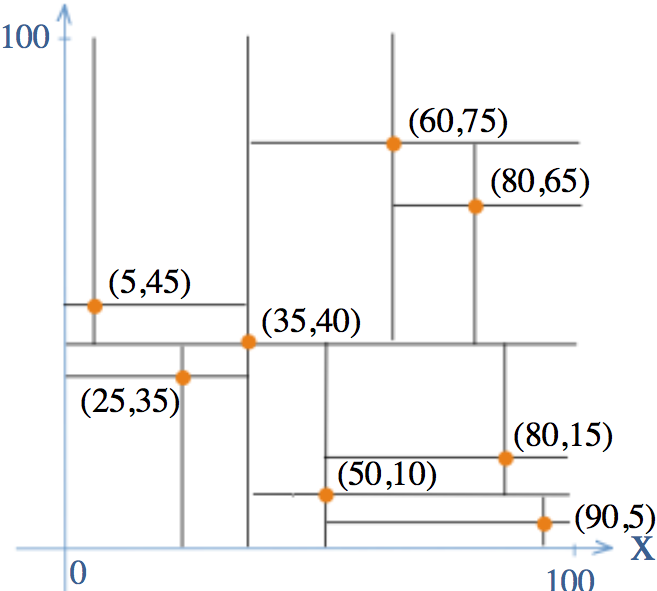
\includegraphics[width=0.4\textwidth]{img/example.png}
					%\caption{Dados vetoriais.}
				\end{figure}
				
				\begin{minipage}{\textwidth}
					\centering
					\footnotesize
					\begin{forest}
						[\texttt{(35,40)}
						[\texttt{(05,45)}
						[x]
						[x]
						[x]
						[x]
						]
						[\texttt{(60,75)}
						[x]
						[x]
						[x]
						[\texttt{(80,65)}]
						]
						[\texttt{(25,35)}
						[x]
						[x]
						[x]
						[x]
						]
						[\texttt{(50,10)}
						[x]
						[\texttt{(85,15)}]
						[x]
						[\texttt{(90,05)}]
						]
						]
					\end{forest}
				\end{minipage}
			\end{frame}

			\begin{frame}[fragile]
				\begin{algorithm2e}[H]
					\tcp{Inicia-se pela raiz}
					\If{    $x\_Baixo <= x$ e $x <= x\_Alto$ 
								e 
							$y\_Baixo <= y$ e $y <= y\_Alto$}{Adiciona o ponto ao vetor de pontos\;}
					\If{$x\_Baixo <= x$ e $y\_Baixo <= y$}{Sudoeste\;}
					\If{$x\_Baixo <= x$ e $y <  y\_Alto$}{Noroeste\;}
					\If{$x >  x\_Alto$ e $y\_Baixo <= x$}{Sudeste\;}
					\If{$x >  x\_Alto$ e $y <=  y\_Alto$}{Nordeste\;}
					\caption{Interval Search - $\mathcal{O}(\log_4 n)$} 
				\end{algorithm2e}
			\end{frame}

			\begin{frame}
				\begin{figure}
					\centering
					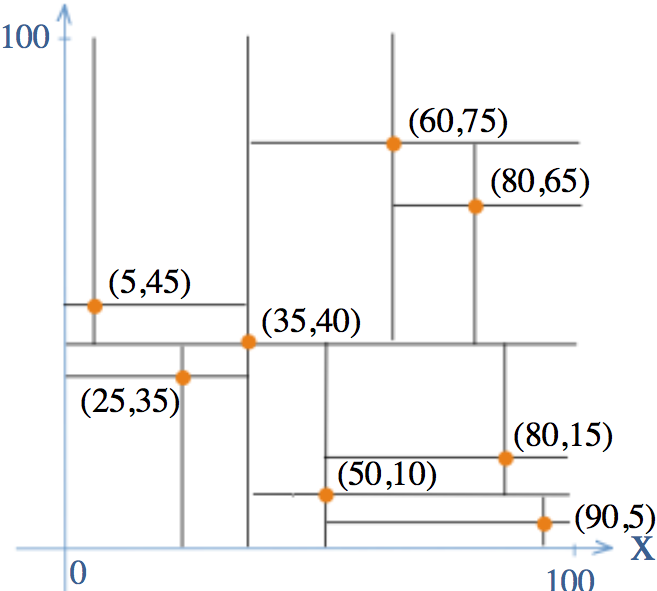
\includegraphics[width=0.5\textwidth]{img/example.png}
					%\caption{Dados vetoriais.}
					
					\vspace{10px}
					
					\fcolorbox{red}{white}{\texttt{(35,40), (50,10), (60,75), (80,65), (85,15), (05,45), (25,35), (90,05)}}
				\end{figure}
			\end{frame}

			\begin{frame}
				\begin{figure}
					\centering
					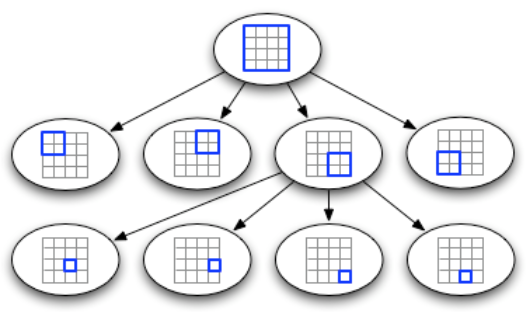
\includegraphics[width=0.8\textwidth]{img/introducao.png}	
				\end{figure}
			\end{frame}

			\begin{frame}[fragile]{Registro em C}
				\begin{minted}{c}
int retorna_quadrante(PQNo *p, PQNo *r) 
{
	if (p->x < r->x)
		if (p->y < r->y)
			return SO;
		else
			return SE;
	else
		if (p->y < r->y)
			return NO;
	else
			return NE;
}
				\end{minted}
			\end{frame}

			\begin{frame}[fragile]{Insere na Point QuadTree em C}
				\begin{minted}{c}
PQNo *PtInsere(PQNo **raiz, PQNo *p) {
	PQNo *f, *r; int q;
	// Arvore esta vazia, então insere
	if (*raiz == NULL) { *raiz = p; return p; } 
	// Desce na árvore até encontrar um quad. vazio ou um ponto igual
	r = *raiz;
	while((r != NULL) && !(r->x == p->x  &&  r->y == p->y)) {
		f = r;	               // Guarda o pai 
		q = retorna_quadrante(p, r); // Descobre o quadrante
		r = r->filhos[q];           // Define nova raiz
	}
	// Verifica se já existe filho
	if (r == NULL) { f->filhos[q] = p; return p; }
	return NULL; // Caso já exista
}
				\end{minted}
			\end{frame}

		\subsubsection{PointRegion-QuadTree}

			\begin{frame}{PointRegion-QuadTree}
				\vspace{-20px}
				\begin{columns}
					\begin{column}{0.48\textwidth}
						\begin{figure}
							\centering
							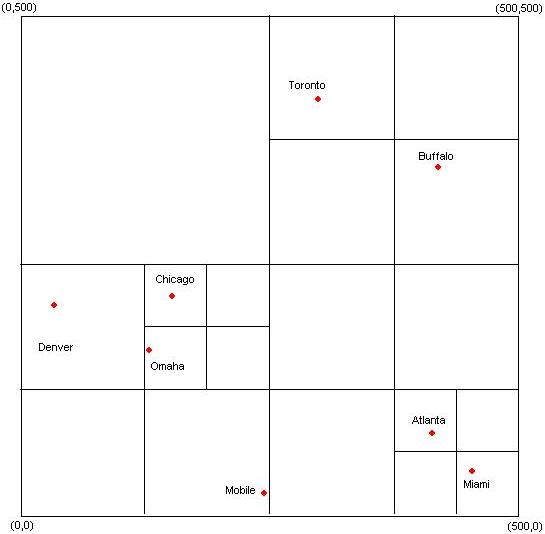
\includegraphics[width=1\textwidth]{img/prquad_q.jpg}
							%\caption{Dados vetoriais.}
						\end{figure}
					\end{column}
					\begin{column}{0.5\textwidth}
						\begin{figure}
							\centering
							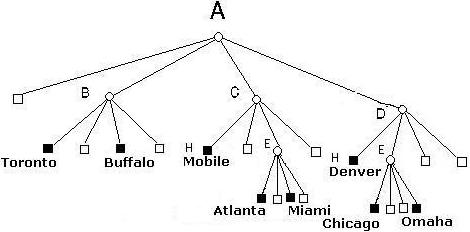
\includegraphics[width=1\textwidth]{img/prquad_t.jpg}
							%\caption{Dados vetoriais.}
						\end{figure}
					\end{column}
				\end{columns}
			\end{frame}

			\begin{frame}{PointRegion-QuadTree}
				\begin{figure}
					\centering
					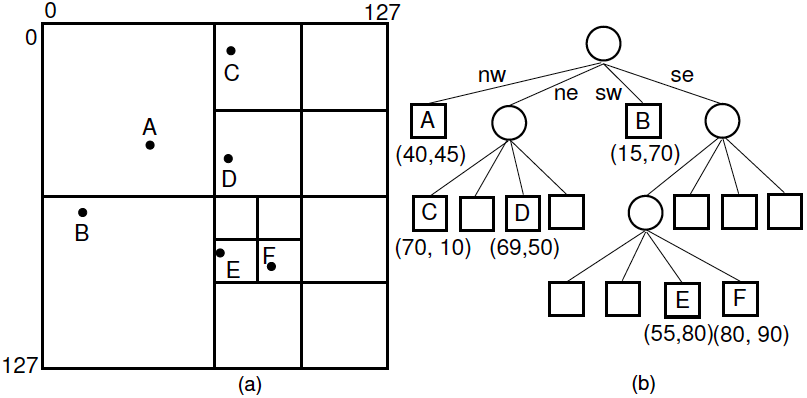
\includegraphics[width=0.9\textwidth]{img/quad_tree_f.png}
				\end{figure}
			\end{frame}

			\begin{frame}{PointRegion-QuadTree}
				\begin{figure}
					\centering
					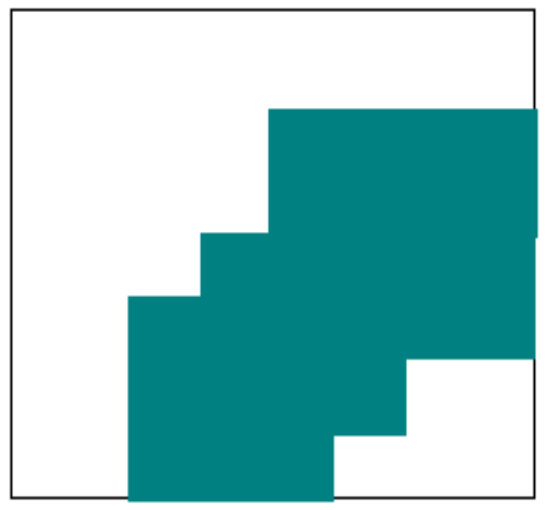
\includegraphics[width=0.5\textwidth]{img/pf_1.png}
					%\caption{Dados vetoriais.}
				\end{figure}
			\end{frame}
			
			\begin{frame}{PointRegion-QuadTree}
				\begin{figure}
					\centering
					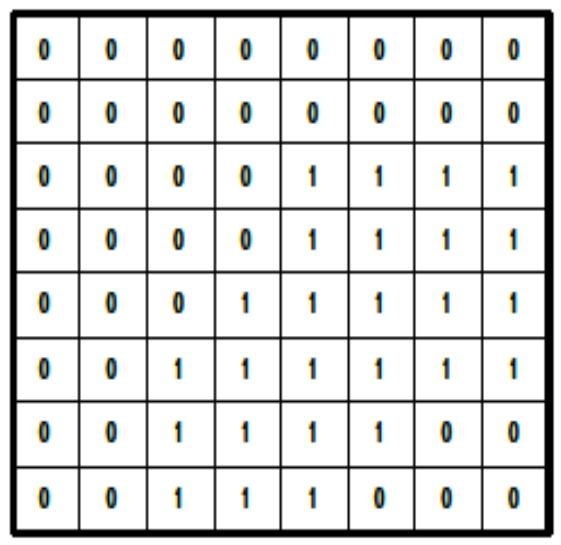
\includegraphics[width=0.5\textwidth]{img/pf_2.png}
					%\caption{Dados vetoriais.}
				\end{figure}
			\end{frame}
			
			\begin{frame}{PointRegion-QuadTree}
				\begin{figure}
					\centering
					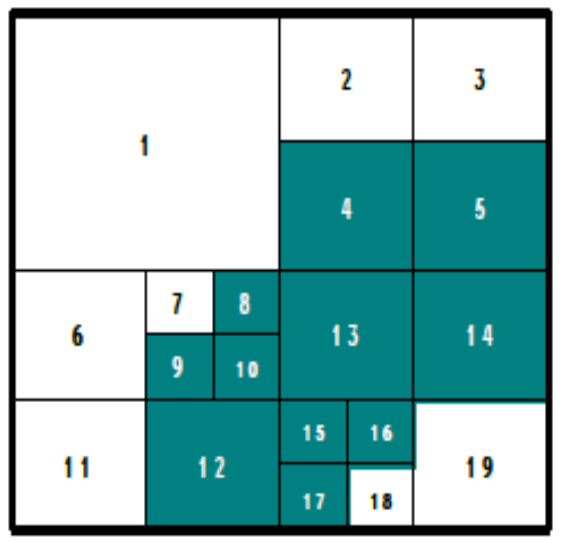
\includegraphics[width=0.5\textwidth]{img/pf_3.png}
					%\caption{Dados vetoriais.}
				\end{figure}
			\end{frame}
			
			\begin{frame}{PointRegion-QuadTree}
				\begin{figure}
					\centering
					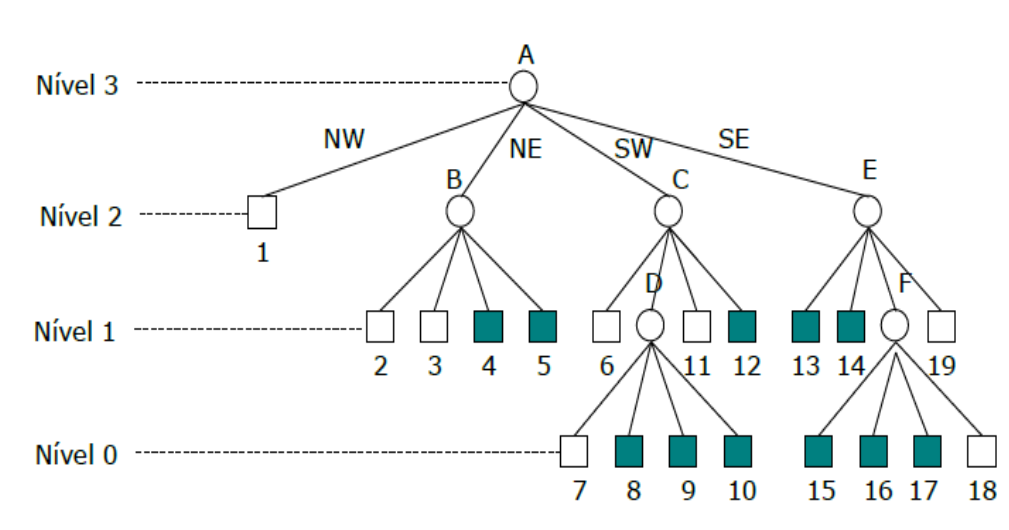
\includegraphics[width=0.9\textwidth]{img/pf_4.png}
					%\caption{Dados vetoriais.}
				\end{figure}
			\end{frame}
			
			\begin{frame}{PointRegion-QuadTree}
				\begin{figure}
					\centering
					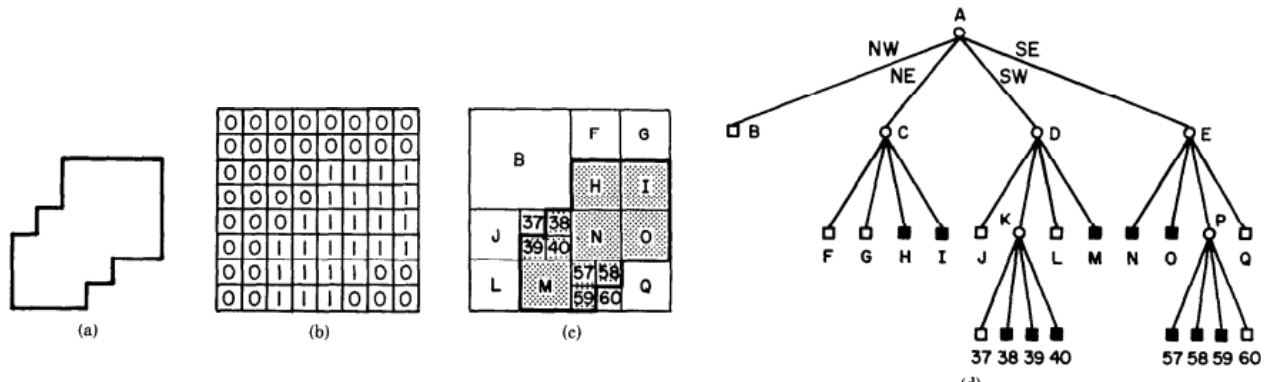
\includegraphics[width=1\textwidth]{img/pf_5.png}
					%\caption{Dados vetoriais.}
				\end{figure}
			\end{frame}
			
			\begin{frame}[fragile]
				\begin{algorithm2e}[H]
					\tcp{Inicia-se pela raiz}
					\uIf{Se a raiz é nula}{
						Cria-se a raiz\;
						Insere Ponto no filho correspondente\;}
					\uElseIf{Se a posição está nula}{Insere Ponto no local correspondente\;}
					\ElseIf{Se a página já possuir um Ponto na posição}{
						Adicione o nó já situado numa nova sub-árvore desta raiz\;
						Realize a verificação novamente com o nó a ser inserido\;}
						\caption{Insertion PR-QuadTree} 
				\end{algorithm2e}
			\end{frame}
			
			\begin{frame}[fragile]{Point QuadTree}{Exemplo Prático}
				\centering
				\vspace{-40px}
				\begin{columns}
					\begin{column}{0.48\textwidth}
						\begin{figure}
							\centering
							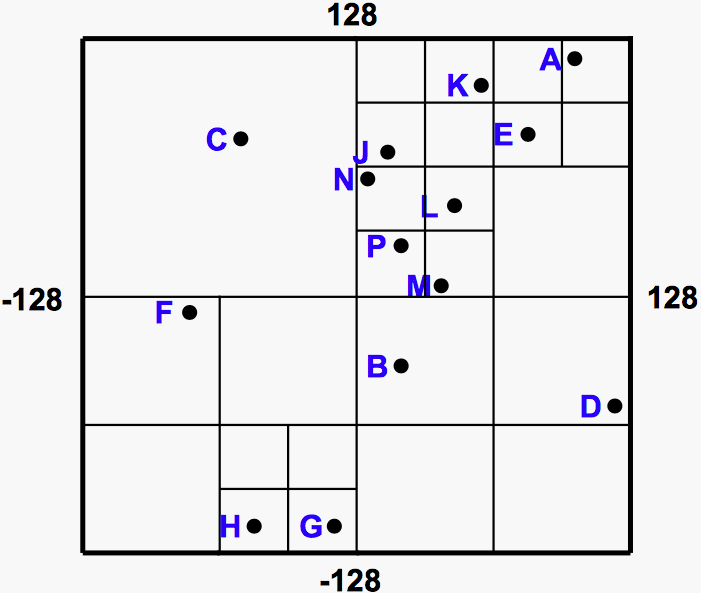
\includegraphics[width=1\textwidth]{img/pr-quad.png}
							%\caption{Dados vetoriais.}
						\end{figure}
					\end{column}
					\begin{column}{0.5\textwidth}
						\centering
						\fbox{
							\begin{forest}
								[\texttt{(x,y)}
								[NO]
								[NE]
								[SO]
								[SE]
								]
						\end{forest}}
							\pause
							
						\begin{forest}
							[x
								[x]
								[\texttt{A}
								]
								[x]
								[x]
							]
						\end{forest}
						
						\end{column}
				\end{columns}
			\end{frame}

			\begin{frame}[fragile]{Point QuadTree}{Exemplo Prático}
				\centering
				\vspace{-40px}
				\begin{columns}
					\begin{column}{0.48\textwidth}
						\begin{figure}
							\centering
							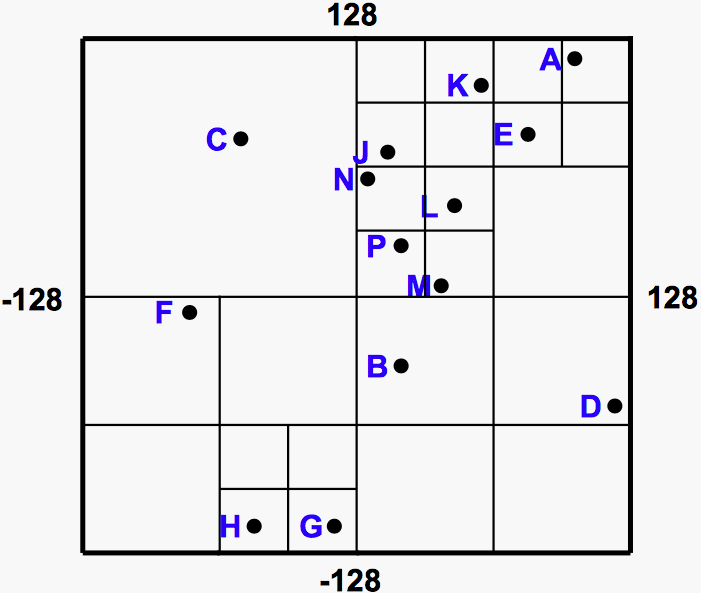
\includegraphics[width=0.9\textwidth]{img/pr-quad.png}
							%\caption{Dados vetoriais.}
						\end{figure}
					\end{column}
					\begin{column}{0.5\textwidth}
						\centering
						\fbox{
							\begin{forest}
								[\texttt{(x,y)}
								[NO]
								[NE]
								[SO]
								[SE]
								]
						\end{forest}}
						
						\begin{forest}
							[x
							[x]
							[\texttt{A}
							]
							[x]
							[\texttt{B}]
							]
						\end{forest}
					\end{column}
				\end{columns}
			\end{frame}
			
			
			\begin{frame}[fragile]{Point QuadTree}{Exemplo Prático}
				\centering
				\vspace{-40px}
				\begin{columns}
					\begin{column}{0.48\textwidth}
						\begin{figure}
							\centering
							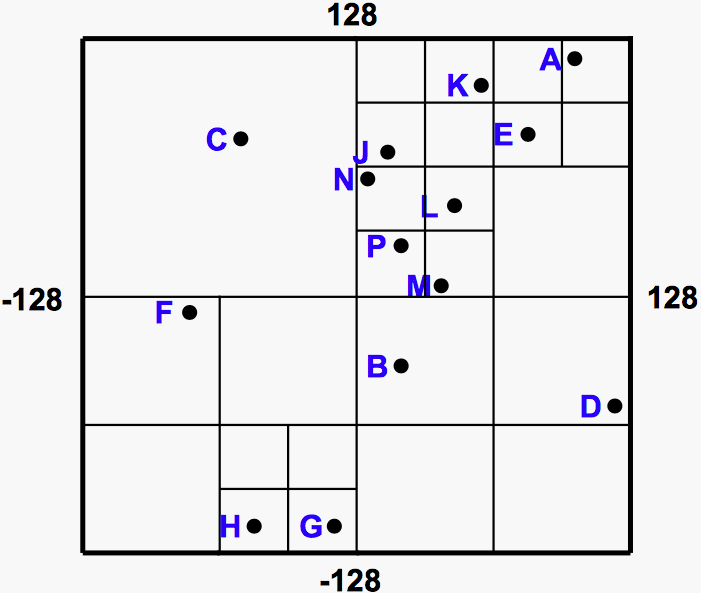
\includegraphics[width=0.9\textwidth]{img/pr-quad.png}
							%\caption{Dados vetoriais.}
						\end{figure}
					\end{column}
					\begin{column}{0.5\textwidth}
						\centering
						\fbox{
							\begin{forest}
								[\texttt{(x,y)}
								[NO]
								[NE]
								[SO]
								[SE]
								]
						\end{forest}}
						
						\begin{forest}
							[x
							[\texttt{C}
							]
							[\texttt{A}
							]
							[x]
							[\texttt{B}]
							]
						\end{forest}
						
						
					\end{column}
				\end{columns}
			\end{frame}
			
			
			\begin{frame}[fragile]{Point QuadTree}{Exemplo Prático}
				\centering
				\vspace{-40px}
				\begin{columns}
					\begin{column}{0.48\textwidth}
						\begin{figure}
							\centering
							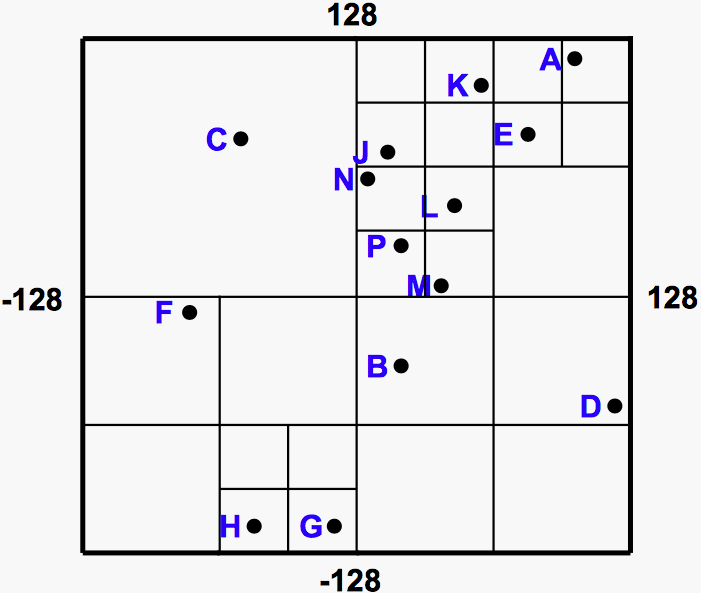
\includegraphics[width=0.9\textwidth]{img/pr-quad.png}
							%\caption{Dados vetoriais.}
						\end{figure}
					\end{column}
					\begin{column}{0.5\textwidth}
						\centering
						\fbox{
							\begin{forest}
								[\texttt{(x,y)}
								[NO]
								[NE]
								[SO]
								[SE]
								]
						\end{forest}}
						
						\begin{forest}
							[x
							[\texttt{C}
							]
							[\texttt{A}
							]
							[x]
							[x
							[\texttt{B}]
							[\texttt{D}]
							[x]
							[x]
							]
							]
						\end{forest}
						
					\end{column}
				\end{columns}
			\end{frame}
			
			
			
			\begin{frame}[fragile]{Point QuadTree}{Exemplo Prático}
				\centering
				\vspace{-40px}
				\begin{columns}
					\begin{column}{0.48\textwidth}
						\begin{figure}
							\centering
							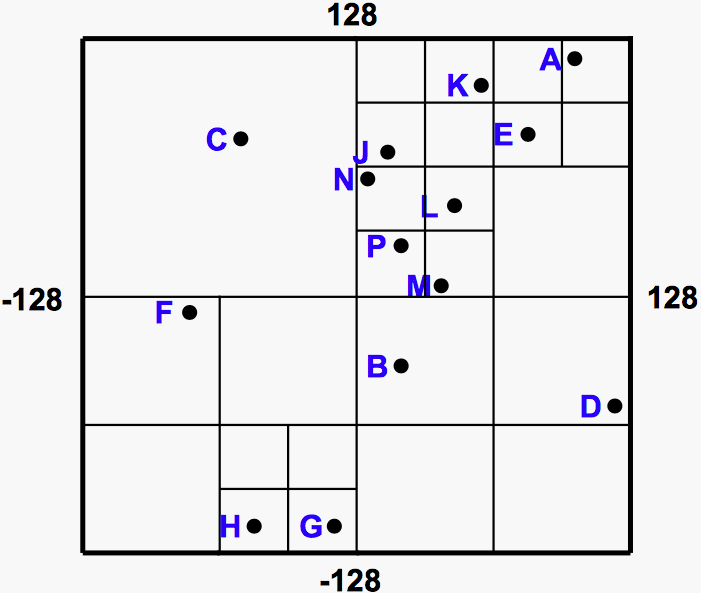
\includegraphics[width=0.9\textwidth]{img/pr-quad.png}
							%\caption{Dados vetoriais.}
						\end{figure}
					\end{column}
					\begin{column}{0.5\textwidth}
						\centering
						\fbox{
							\begin{forest}
								[\texttt{(x,y)}
								[NO]
								[NE]
								[SO]
								[SE]
								]
						\end{forest}}
						
						\begin{forest}
							[x
							[\texttt{C}
							]
							[x
								[x]
								[x
									[x]
									[\texttt{A}]
									[\texttt{E}]
									[x]
								]
								[x]
								[x]
							]
							[x]
							[x
							[\texttt{B}]
							[\texttt{D}]
							[x]
							[x]
							]
							]
						\end{forest}
						
					\end{column}
				\end{columns}
			\end{frame}
			
			
			\begin{frame}[fragile]{Point QuadTree}{Exemplo Prático}
				\centering
				\vspace{-40px}
				\begin{columns}
					\begin{column}{0.48\textwidth}
						\begin{figure}
							\centering
							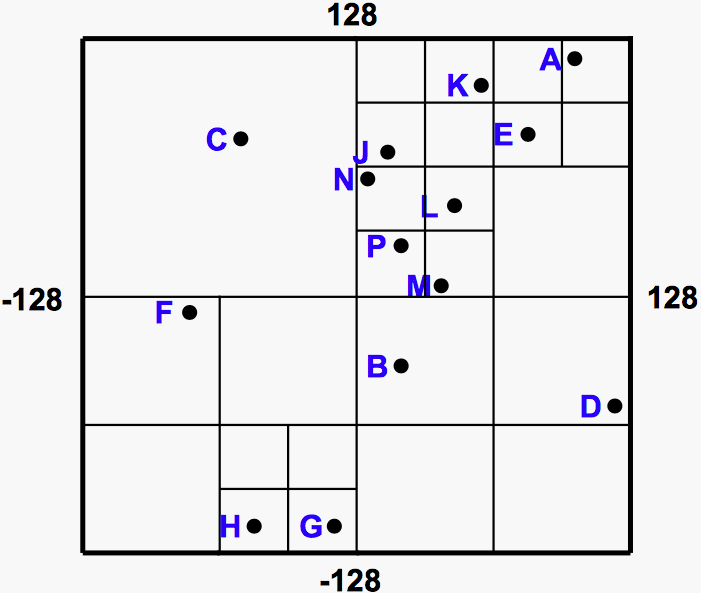
\includegraphics[width=0.9\textwidth]{img/pr-quad.png}
							%\caption{Dados vetoriais.}
						\end{figure}
					\end{column}
					\begin{column}{0.5\textwidth}
						\centering
						\fbox{
							\begin{forest}
								[\texttt{(x,y)}
								[NO]
								[NE]
								[SO]
								[SE]
								]
						\end{forest}}
						
						\begin{forest}
							[x
							[\texttt{C}
							]
							[x
							[x]
							[x
							[x]
							[\texttt{A}]
							[\texttt{E}]
							[x]
							]
							[x]
							[x]
							]
							[\texttt{F}]
							[x
							[\texttt{B}]
							[\texttt{D}]
							[x]
							[x]
							]
							]
						\end{forest}
						
					\end{column}
				\end{columns}
			\end{frame}
			
			
			\begin{frame}[fragile]{Point QuadTree}{Exemplo Prático}
				\centering
				\vspace{-40px}
				\begin{columns}
					\begin{column}{0.4\textwidth}
						\begin{figure}
							\centering
							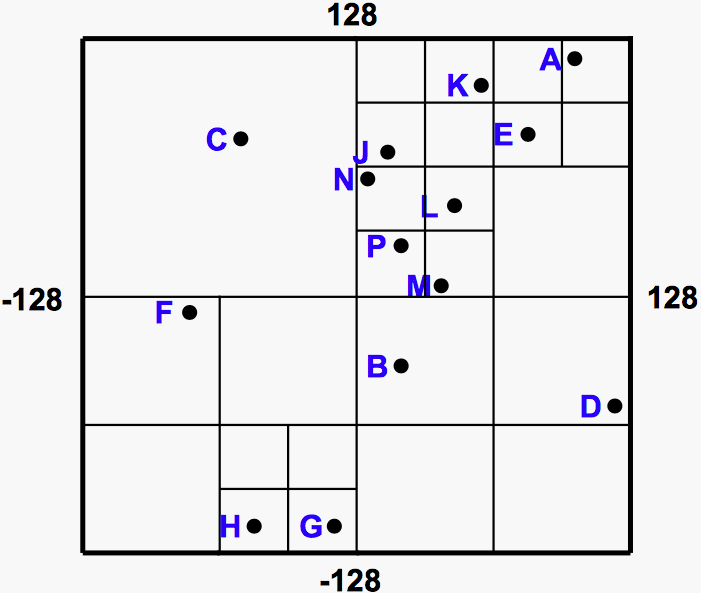
\includegraphics[width=0.8\textwidth]{img/pr-quad.png}
							%\caption{Dados vetoriais.}
						\end{figure}
					\end{column}
					\begin{column}{0.55\textwidth}
						\centering
						\fbox{
							\begin{forest}
								[\texttt{(x,y)}
								[NO]
								[NE]
								[SO]
								[SE]
								]
						\end{forest}}
						
						\begin{forest}
							[x
							[\texttt{C}
							]
							[x
							[x]
							[x
							[x]
							[\texttt{A}]
							[\texttt{E}]
							[x]
							]
							[x]
							[x]
							]
							[x
								[\texttt{F}]
								[x]
								[x]
								[\texttt{G}]
							]
							[x
							[\texttt{B}]
							[\texttt{D}]
							[x]
							[x]
							]
							]
						\end{forest}
						
					\end{column}
				\end{columns}
			\end{frame}


	\subsection{Vantagens e Desvantagens}
	
		\begin{frame}{Vantagens e Desvantagens}
			\begin{columns}
				\begin{column}{0.48\textwidth}
					Vantagens:
					\begin{itemize}
						\item Possui estrutura mais enxuta e robusta que árvores binárias;
						
						\item Inserções não afetam a performance e por isso não necessitam de rebalanceamento.
					\end{itemize}
				\end{column}
				\begin{column}{0.5\textwidth}
					Desvantagens:
					\begin{itemize}
						\setlength{\itemsep}{1em}
						\item Se a imagem a ser compactada tiver muitas cores, a complexidade da árvore pode tornar o arquivo compactado maior que o original;
						
						\item Imagens complexas usam muito de CPU para gerar suas QuadTree;
						
						\item QuadTree funciona somente com imagens de 2 dimensões.
						\begin{itemize}
							\item A R-Tree, por exemplo, trabalha com 4 dimensões.
						\end{itemize}
					\end{itemize}
				\end{column}
			\end{columns}
		\end{frame}

	
	\subsection{Outras Estruturas de Dados Espaciais}
		\begin{frame}{Outras Estruturas de Dados Espaciais}
			\begin{itemize}
				\setlength{\itemsep}{1.2em}
				\item QuadTree;
				\item Grid;
				\item K-d-Tree;
				\item R-Tree.
			\end{itemize}
		\end{frame}

		\begin{frame}{Dúvidas, Sugestões ou Reclamações?}
			\begin{itemize}
				\item \url{rodolfolabiapari@decom.ufop.br} \\[1cm]
				\item \url{https://www.guerrillamail.com/}
			\end{itemize}
		\end{frame}

\frame{\titlepage}

\end{document}
